\section{Methodology}

\begin{enumerate}
	\item 4 shots of grid: 1. LE 2. TE 3. near-field for entire shape 4. the entire grid domain. Note: should show T-rex feature that was used
	\item table 1: cell count and normal-to-wall spacing used, list BC, list reference values, list submodels chosen (i.e. viscous model), provide numerical scheme and spacial accuracy
	
\subsection{Screenshots of grid}

\begin{figure}[H]
	\centering
	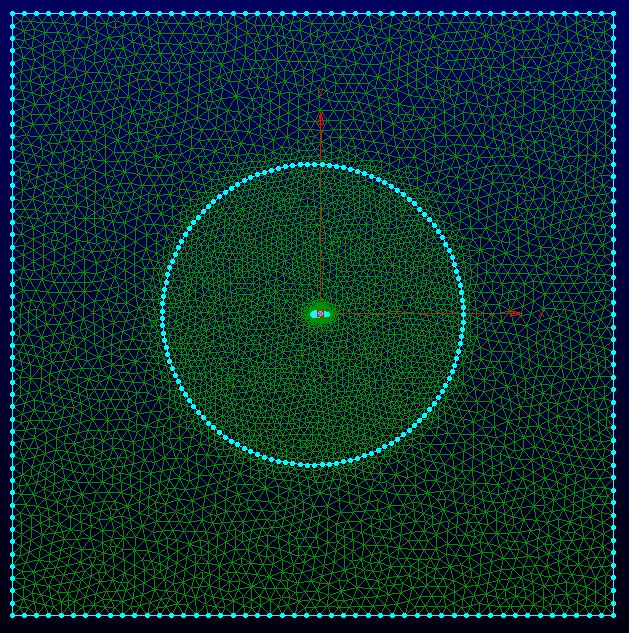
\includegraphics[width=\textwidth]{general_images/farfield}
	\caption{Farfield}
\label{fig:farfield}
\end{figure}

\begin{figure}[H]
	\centering
	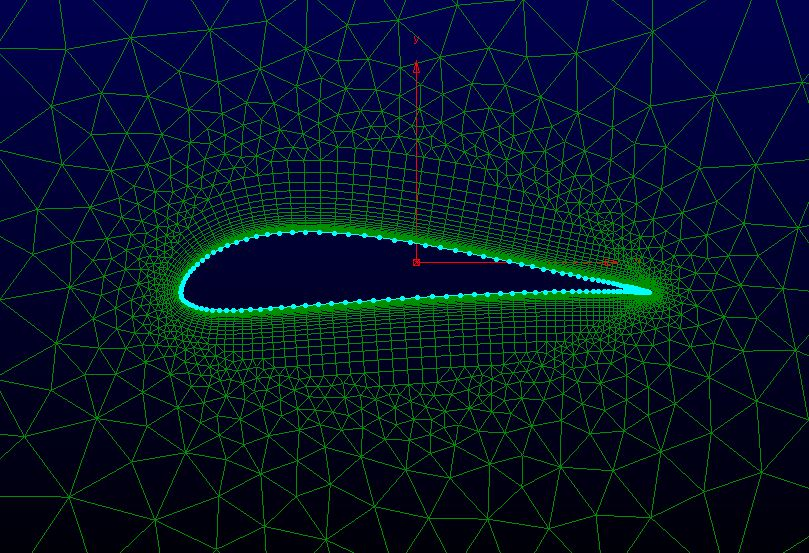
\includegraphics[width=0.9\textwidth]{general_images/nearfield}
	\caption{Nearfield}
\label{fig:nearfield}
\end{figure}	

\begin{figure}[H]
	\centering
	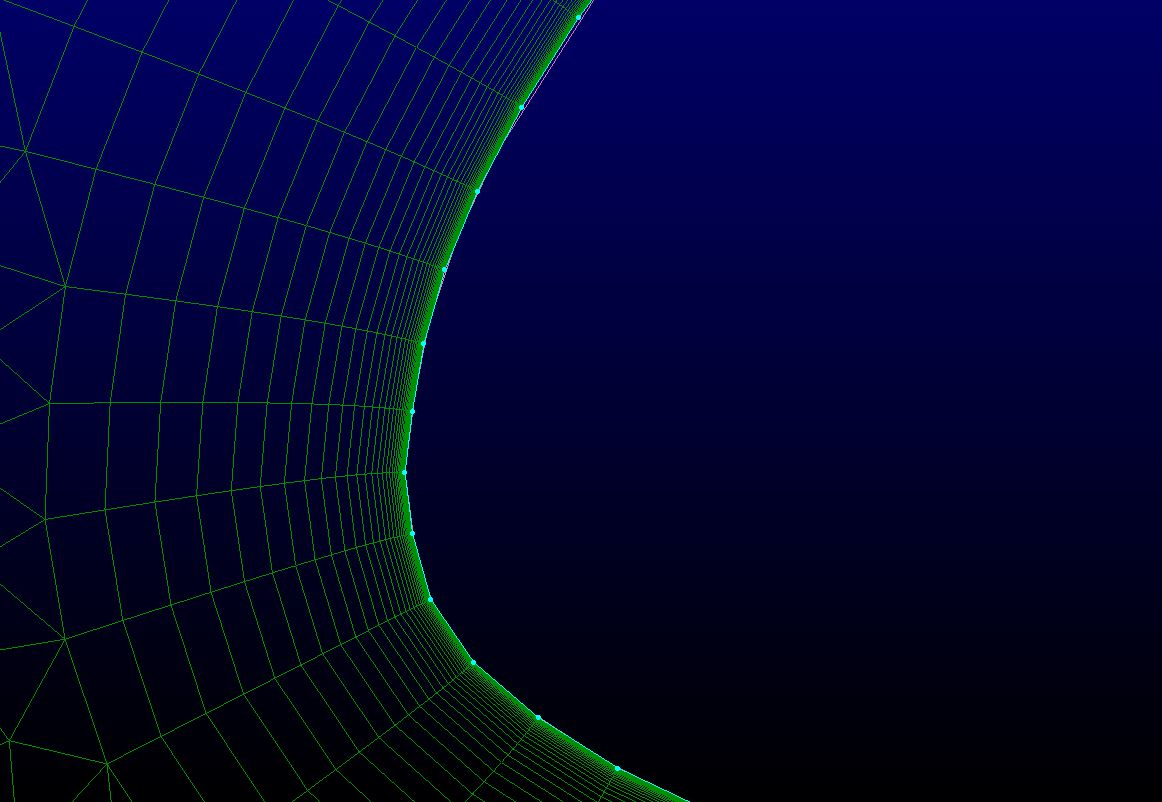
\includegraphics[width=0.9\textwidth]{general_images/LE1}
	\caption{Leading edge}
\label{fig:LE}
\end{figure}

\begin{figure}[H]
	\centering
	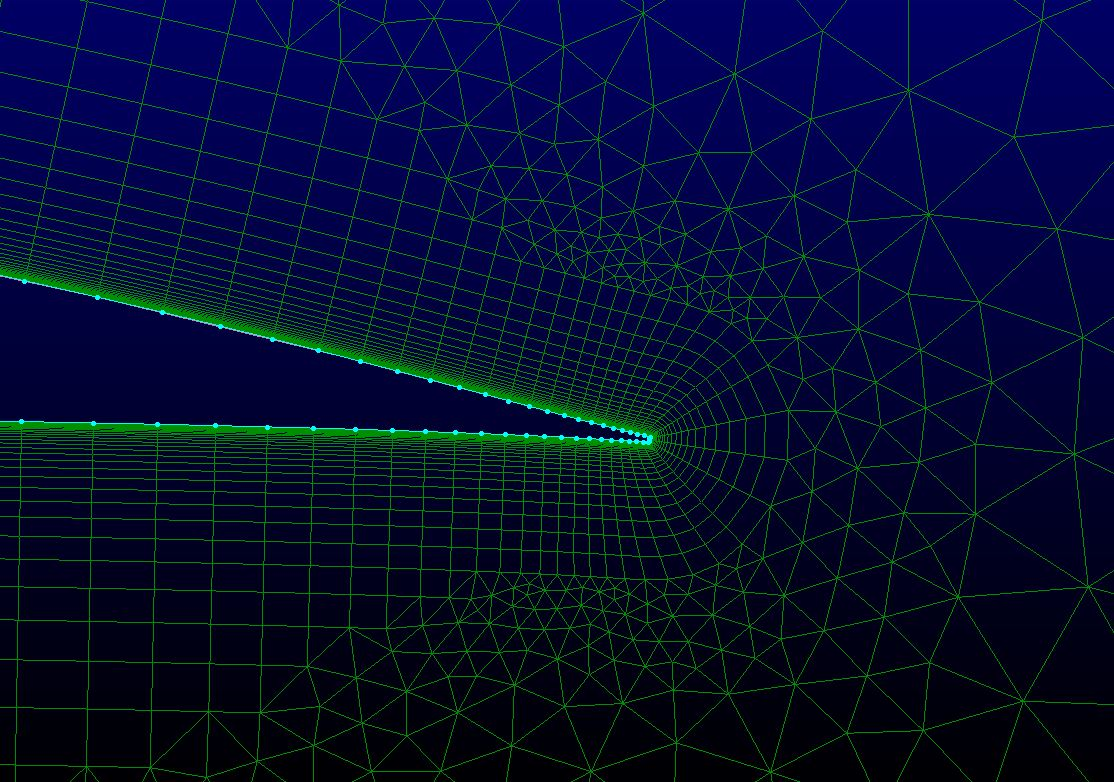
\includegraphics[width=0.9\textwidth]{general_images/TE1}
	\caption{Trailing edge}
\label{fig:TE}
\end{figure}

\begin{table}[H]
\caption{General grid information}
	\centering
	\begin{tabular}{|l|p{4.5in}|} \hline
				 & Value \\ \hline \hline
		Cell count & inner mesh: \newline outer mesh \\ \hline
		Normal-to-wall dist & 1e-5 (UNITS?) \\ \hline
		Boundary condition & airfoil surface: wall, $\Delta$s=1e-5 \newline (might have to specify at inlet and such, check) \\ \hline
		Reference values & A bunch of different ones here, 1.789e-05 kgm$^{-1}$s$^{-1}$ \\ \hline
		Submodels & viscous: transitional SST \\ \hline
		Numerical Schemes & \textbf{gradient}: least-squares cell based \newline \textbf{pressure}: second order \newline \textbf{momentum}: second order upwind \newline \textbf{turbulent kinetic energy}: first order upwind \newline \textbf{specific dissipation rate}: first order upwind \newline \textbf{specific dissipation rate}: first order upwind \newline \textbf{intermittency}: first order upwind \newline \textbf{momentum thickness Re}: first order upwind \\ \hline
	\end{tabular}
\end{table}



% gradient: least squares cell based
% pressure: second order
% momentum: second order upwind
% turbulent kinetic energy: first order upwind
% specific dissipation rate: first order upwind
% intermittency: first order upwind
% momentum thickness Re: first order upwind
		
\end{enumerate}